% Created by tikzDevice version 0.12 on 2019-02-01 11:55:29
% !TEX encoding = UTF-8 Unicode
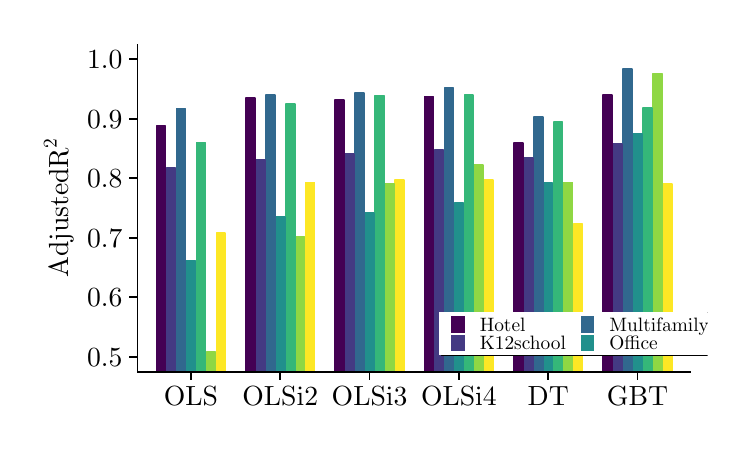
\begin{tikzpicture}[x=1pt,y=1pt]
\definecolor{fillColor}{RGB}{255,255,255}
\path[use as bounding box,fill=fillColor,fill opacity=0.00] (0,0) rectangle (245.72,144.54);
\begin{scope}
\path[clip] (  0.00,  0.00) rectangle (245.72,144.54);
\definecolor{drawColor}{RGB}{255,255,255}
\definecolor{fillColor}{RGB}{255,255,255}

\path[draw=drawColor,line width= 0.6pt,line join=round,line cap=round,fill=fillColor] (  0.00,  0.00) rectangle (245.72,144.54);
\end{scope}
\begin{scope}
\path[clip] ( 39.64, 20.23) rectangle (239.72,138.54);
\definecolor{fillColor}{RGB}{255,255,255}

\path[fill=fillColor] ( 39.64, 20.23) rectangle (239.72,138.54);
\definecolor{drawColor}{RGB}{253,231,37}
\definecolor{fillColor}{RGB}{253,231,37}

\path[draw=drawColor,line width= 0.6pt,line join=round,fill=fillColor] ( 68.18,-81.94) rectangle ( 71.41, 70.35);
\definecolor{drawColor}{RGB}{143,215,68}
\definecolor{fillColor}{RGB}{143,215,68}

\path[draw=drawColor,line width= 0.6pt,line join=round,fill=fillColor] ( 64.58,-81.94) rectangle ( 67.81, 27.33);
\definecolor{drawColor}{RGB}{53,183,121}
\definecolor{fillColor}{RGB}{53,183,121}

\path[draw=drawColor,line width= 0.6pt,line join=round,fill=fillColor] ( 60.99,-81.94) rectangle ( 64.21,103.05);
\definecolor{drawColor}{RGB}{33,144,140}
\definecolor{fillColor}{RGB}{33,144,140}

\path[draw=drawColor,line width= 0.6pt,line join=round,fill=fillColor] ( 57.39,-81.94) rectangle ( 60.62, 60.46);
\definecolor{drawColor}{RGB}{49,104,142}
\definecolor{fillColor}{RGB}{49,104,142}

\path[draw=drawColor,line width= 0.6pt,line join=round,fill=fillColor] ( 53.80,-81.94) rectangle ( 57.02,115.31);
\definecolor{drawColor}{RGB}{68,58,131}
\definecolor{fillColor}{RGB}{68,58,131}

\path[draw=drawColor,line width= 0.6pt,line join=round,fill=fillColor] ( 50.20,-81.94) rectangle ( 53.43, 93.80);
\definecolor{drawColor}{RGB}{68,1,84}
\definecolor{fillColor}{RGB}{68,1,84}

\path[draw=drawColor,line width= 0.6pt,line join=round,fill=fillColor] ( 46.60,-81.94) rectangle ( 49.83,109.07);
\definecolor{drawColor}{RGB}{253,231,37}
\definecolor{fillColor}{RGB}{253,231,37}

\path[draw=drawColor,line width= 0.6pt,line join=round,fill=fillColor] (100.45,-81.94) rectangle (103.68, 88.64);
\definecolor{drawColor}{RGB}{143,215,68}
\definecolor{fillColor}{RGB}{143,215,68}

\path[draw=drawColor,line width= 0.6pt,line join=round,fill=fillColor] ( 96.85,-81.94) rectangle (100.08, 69.06);
\definecolor{drawColor}{RGB}{53,183,121}
\definecolor{fillColor}{RGB}{53,183,121}

\path[draw=drawColor,line width= 0.6pt,line join=round,fill=fillColor] ( 93.26,-81.94) rectangle ( 96.48,117.03);
\definecolor{drawColor}{RGB}{33,144,140}
\definecolor{fillColor}{RGB}{33,144,140}

\path[draw=drawColor,line width= 0.6pt,line join=round,fill=fillColor] ( 89.66,-81.94) rectangle ( 92.89, 76.16);
\definecolor{drawColor}{RGB}{49,104,142}
\definecolor{fillColor}{RGB}{49,104,142}

\path[draw=drawColor,line width= 0.6pt,line join=round,fill=fillColor] ( 86.07,-81.94) rectangle ( 89.29,120.26);
\definecolor{drawColor}{RGB}{68,58,131}
\definecolor{fillColor}{RGB}{68,58,131}

\path[draw=drawColor,line width= 0.6pt,line join=round,fill=fillColor] ( 82.47,-81.94) rectangle ( 85.70, 96.81);
\definecolor{drawColor}{RGB}{68,1,84}
\definecolor{fillColor}{RGB}{68,1,84}

\path[draw=drawColor,line width= 0.6pt,line join=round,fill=fillColor] ( 78.87,-81.94) rectangle ( 82.10,119.18);
\definecolor{drawColor}{RGB}{253,231,37}
\definecolor{fillColor}{RGB}{253,231,37}

\path[draw=drawColor,line width= 0.6pt,line join=round,fill=fillColor] (132.72,-81.94) rectangle (135.95, 89.50);
\definecolor{drawColor}{RGB}{143,215,68}
\definecolor{fillColor}{RGB}{143,215,68}

\path[draw=drawColor,line width= 0.6pt,line join=round,fill=fillColor] (129.12,-81.94) rectangle (132.35, 88.20);
\definecolor{drawColor}{RGB}{53,183,121}
\definecolor{fillColor}{RGB}{53,183,121}

\path[draw=drawColor,line width= 0.6pt,line join=round,fill=fillColor] (125.53,-81.94) rectangle (128.75,120.04);
\definecolor{drawColor}{RGB}{33,144,140}
\definecolor{fillColor}{RGB}{33,144,140}

\path[draw=drawColor,line width= 0.6pt,line join=round,fill=fillColor] (121.93,-81.94) rectangle (125.16, 77.66);
\definecolor{drawColor}{RGB}{49,104,142}
\definecolor{fillColor}{RGB}{49,104,142}

\path[draw=drawColor,line width= 0.6pt,line join=round,fill=fillColor] (118.34,-81.94) rectangle (121.56,120.90);
\definecolor{drawColor}{RGB}{68,58,131}
\definecolor{fillColor}{RGB}{68,58,131}

\path[draw=drawColor,line width= 0.6pt,line join=round,fill=fillColor] (114.74,-81.94) rectangle (117.97, 98.96);
\definecolor{drawColor}{RGB}{68,1,84}
\definecolor{fillColor}{RGB}{68,1,84}

\path[draw=drawColor,line width= 0.6pt,line join=round,fill=fillColor] (111.14,-81.94) rectangle (114.37,118.32);
\definecolor{drawColor}{RGB}{253,231,37}
\definecolor{fillColor}{RGB}{253,231,37}

\path[draw=drawColor,line width= 0.6pt,line join=round,fill=fillColor] (164.99,-81.94) rectangle (168.22, 89.50);
\definecolor{drawColor}{RGB}{143,215,68}
\definecolor{fillColor}{RGB}{143,215,68}

\path[draw=drawColor,line width= 0.6pt,line join=round,fill=fillColor] (161.39,-81.94) rectangle (164.62, 94.87);
\definecolor{drawColor}{RGB}{53,183,121}
\definecolor{fillColor}{RGB}{53,183,121}

\path[draw=drawColor,line width= 0.6pt,line join=round,fill=fillColor] (157.80,-81.94) rectangle (161.02,120.26);
\definecolor{drawColor}{RGB}{33,144,140}
\definecolor{fillColor}{RGB}{33,144,140}

\path[draw=drawColor,line width= 0.6pt,line join=round,fill=fillColor] (154.20,-81.94) rectangle (157.43, 81.11);
\definecolor{drawColor}{RGB}{49,104,142}
\definecolor{fillColor}{RGB}{49,104,142}

\path[draw=drawColor,line width= 0.6pt,line join=round,fill=fillColor] (150.61,-81.94) rectangle (153.83,122.62);
\definecolor{drawColor}{RGB}{68,58,131}
\definecolor{fillColor}{RGB}{68,58,131}

\path[draw=drawColor,line width= 0.6pt,line join=round,fill=fillColor] (147.01,-81.94) rectangle (150.24,100.25);
\definecolor{drawColor}{RGB}{68,1,84}
\definecolor{fillColor}{RGB}{68,1,84}

\path[draw=drawColor,line width= 0.6pt,line join=round,fill=fillColor] (143.41,-81.94) rectangle (146.64,119.61);
\definecolor{drawColor}{RGB}{253,231,37}
\definecolor{fillColor}{RGB}{253,231,37}

\path[draw=drawColor,line width= 0.6pt,line join=round,fill=fillColor] (197.26,-81.94) rectangle (200.49, 73.58);
\definecolor{drawColor}{RGB}{143,215,68}
\definecolor{fillColor}{RGB}{143,215,68}

\path[draw=drawColor,line width= 0.6pt,line join=round,fill=fillColor] (193.66,-81.94) rectangle (196.89, 88.64);
\definecolor{drawColor}{RGB}{53,183,121}
\definecolor{fillColor}{RGB}{53,183,121}

\path[draw=drawColor,line width= 0.6pt,line join=round,fill=fillColor] (190.07,-81.94) rectangle (193.29,110.36);
\definecolor{drawColor}{RGB}{33,144,140}
\definecolor{fillColor}{RGB}{33,144,140}

\path[draw=drawColor,line width= 0.6pt,line join=round,fill=fillColor] (186.47,-81.94) rectangle (189.70, 88.42);
\definecolor{drawColor}{RGB}{49,104,142}
\definecolor{fillColor}{RGB}{49,104,142}

\path[draw=drawColor,line width= 0.6pt,line join=round,fill=fillColor] (182.88,-81.94) rectangle (186.10,112.30);
\definecolor{drawColor}{RGB}{68,58,131}
\definecolor{fillColor}{RGB}{68,58,131}

\path[draw=drawColor,line width= 0.6pt,line join=round,fill=fillColor] (179.28,-81.94) rectangle (182.51, 97.45);
\definecolor{drawColor}{RGB}{68,1,84}
\definecolor{fillColor}{RGB}{68,1,84}

\path[draw=drawColor,line width= 0.6pt,line join=round,fill=fillColor] (175.68,-81.94) rectangle (178.91,102.83);
\definecolor{drawColor}{RGB}{253,231,37}
\definecolor{fillColor}{RGB}{253,231,37}

\path[draw=drawColor,line width= 0.6pt,line join=round,fill=fillColor] (229.53,-81.94) rectangle (232.76, 87.99);
\definecolor{drawColor}{RGB}{143,215,68}
\definecolor{fillColor}{RGB}{143,215,68}

\path[draw=drawColor,line width= 0.6pt,line join=round,fill=fillColor] (225.93,-81.94) rectangle (229.16,128.00);
\definecolor{drawColor}{RGB}{53,183,121}
\definecolor{fillColor}{RGB}{53,183,121}

\path[draw=drawColor,line width= 0.6pt,line join=round,fill=fillColor] (222.34,-81.94) rectangle (225.57,115.52);
\definecolor{drawColor}{RGB}{33,144,140}
\definecolor{fillColor}{RGB}{33,144,140}

\path[draw=drawColor,line width= 0.6pt,line join=round,fill=fillColor] (218.74,-81.94) rectangle (221.97,106.27);
\definecolor{drawColor}{RGB}{49,104,142}
\definecolor{fillColor}{RGB}{49,104,142}

\path[draw=drawColor,line width= 0.6pt,line join=round,fill=fillColor] (215.15,-81.94) rectangle (218.37,129.72);
\definecolor{drawColor}{RGB}{68,58,131}
\definecolor{fillColor}{RGB}{68,58,131}

\path[draw=drawColor,line width= 0.6pt,line join=round,fill=fillColor] (211.55,-81.94) rectangle (214.78,102.40);
\definecolor{drawColor}{RGB}{68,1,84}
\definecolor{fillColor}{RGB}{68,1,84}

\path[draw=drawColor,line width= 0.6pt,line join=round,fill=fillColor] (207.95,-81.94) rectangle (211.18,120.26);
\end{scope}
\begin{scope}
\path[clip] (  0.00,  0.00) rectangle (245.72,144.54);
\definecolor{drawColor}{RGB}{0,0,0}

\path[draw=drawColor,line width= 0.6pt,line join=round] ( 39.64, 20.23) --
	( 39.64,138.54);
\end{scope}
\begin{scope}
\path[clip] (  0.00,  0.00) rectangle (245.72,144.54);
\definecolor{drawColor}{RGB}{0,0,0}

\node[text=drawColor,anchor=base east,inner sep=0pt, outer sep=0pt, scale=  1.00] at ( 34.24, 22.17) {0.5};

\node[text=drawColor,anchor=base east,inner sep=0pt, outer sep=0pt, scale=  1.00] at ( 34.24, 43.68) {0.6};

\node[text=drawColor,anchor=base east,inner sep=0pt, outer sep=0pt, scale=  1.00] at ( 34.24, 65.19) {0.7};

\node[text=drawColor,anchor=base east,inner sep=0pt, outer sep=0pt, scale=  1.00] at ( 34.24, 86.70) {0.8};

\node[text=drawColor,anchor=base east,inner sep=0pt, outer sep=0pt, scale=  1.00] at ( 34.24,108.21) {0.9};

\node[text=drawColor,anchor=base east,inner sep=0pt, outer sep=0pt, scale=  1.00] at ( 34.24,129.72) {1.0};
\end{scope}
\begin{scope}
\path[clip] (  0.00,  0.00) rectangle (245.72,144.54);
\definecolor{drawColor}{RGB}{0,0,0}

\path[draw=drawColor,line width= 0.6pt,line join=round] ( 36.64, 25.61) --
	( 39.64, 25.61);

\path[draw=drawColor,line width= 0.6pt,line join=round] ( 36.64, 47.12) --
	( 39.64, 47.12);

\path[draw=drawColor,line width= 0.6pt,line join=round] ( 36.64, 68.63) --
	( 39.64, 68.63);

\path[draw=drawColor,line width= 0.6pt,line join=round] ( 36.64, 90.14) --
	( 39.64, 90.14);

\path[draw=drawColor,line width= 0.6pt,line join=round] ( 36.64,111.65) --
	( 39.64,111.65);

\path[draw=drawColor,line width= 0.6pt,line join=round] ( 36.64,133.16) --
	( 39.64,133.16);
\end{scope}
\begin{scope}
\path[clip] (  0.00,  0.00) rectangle (245.72,144.54);
\definecolor{drawColor}{RGB}{0,0,0}

\path[draw=drawColor,line width= 0.6pt,line join=round] ( 39.64, 20.23) --
	(239.72, 20.23);
\end{scope}
\begin{scope}
\path[clip] (  0.00,  0.00) rectangle (245.72,144.54);
\definecolor{drawColor}{RGB}{0,0,0}

\path[draw=drawColor,line width= 0.6pt,line join=round] ( 59.00, 17.23) --
	( 59.00, 20.23);

\path[draw=drawColor,line width= 0.6pt,line join=round] ( 91.27, 17.23) --
	( 91.27, 20.23);

\path[draw=drawColor,line width= 0.6pt,line join=round] (123.55, 17.23) --
	(123.55, 20.23);

\path[draw=drawColor,line width= 0.6pt,line join=round] (155.82, 17.23) --
	(155.82, 20.23);

\path[draw=drawColor,line width= 0.6pt,line join=round] (188.09, 17.23) --
	(188.09, 20.23);

\path[draw=drawColor,line width= 0.6pt,line join=round] (220.36, 17.23) --
	(220.36, 20.23);
\end{scope}
\begin{scope}
\path[clip] (  0.00,  0.00) rectangle (245.72,144.54);
\definecolor{drawColor}{RGB}{0,0,0}

\node[text=drawColor,anchor=base,inner sep=0pt, outer sep=0pt, scale=  1.00] at ( 59.00,  7.94) {OLS};

\node[text=drawColor,anchor=base,inner sep=0pt, outer sep=0pt, scale=  1.00] at ( 91.27,  7.94) {OLSi2};

\node[text=drawColor,anchor=base,inner sep=0pt, outer sep=0pt, scale=  1.00] at (123.55,  7.94) {OLSi3};

\node[text=drawColor,anchor=base,inner sep=0pt, outer sep=0pt, scale=  1.00] at (155.82,  7.94) {OLSi4};

\node[text=drawColor,anchor=base,inner sep=0pt, outer sep=0pt, scale=  1.00] at (188.09,  7.94) {DT};

\node[text=drawColor,anchor=base,inner sep=0pt, outer sep=0pt, scale=  1.00] at (220.36,  7.94) {GBT};
\end{scope}
\begin{scope}
\path[clip] (  0.00,  0.00) rectangle (245.72,144.54);
\definecolor{drawColor}{RGB}{0,0,0}

\node[text=drawColor,rotate= 90.00,anchor=base west,inner sep=0pt, outer sep=0pt, scale=  1.00] at ( 14.58, 54.35) {Adjusted };

\node[text=drawColor,rotate= 90.00,anchor=base west,inner sep=0pt, outer sep=0pt, scale=  1.00] at ( 14.58, 93.56) {R};

\node[text=drawColor,rotate= 90.00,anchor=base west,inner sep=0pt, outer sep=0pt, scale=  0.70] at ( 10.49,100.92) {2};
\end{scope}
\begin{scope}
\path[clip] (  0.00,  0.00) rectangle (245.72,144.54);
\definecolor{drawColor}{RGB}{0,0,0}

\path[draw=drawColor,line width= 0.4pt,line join=round,line cap=round] (149.68, 26.15) rectangle (336.99, 41.68);
\end{scope}
\begin{scope}
\path[clip] (  0.00,  0.00) rectangle (245.72,144.54);
\definecolor{fillColor}{RGB}{255,255,255}

\path[fill=fillColor] (148.68, 26.15) rectangle (336.99, 41.68);
\end{scope}
\begin{scope}
\path[clip] (  0.00,  0.00) rectangle (245.72,144.54);
\definecolor{drawColor}{RGB}{68,1,84}
\definecolor{fillColor}{RGB}{68,1,84}

\path[draw=drawColor,line width= 0.6pt,line cap=round,fill=fillColor] (153.40, 34.62) rectangle (157.66, 39.97);
\end{scope}
\begin{scope}
\path[clip] (  0.00,  0.00) rectangle (245.72,144.54);
\definecolor{drawColor}{RGB}{68,58,131}
\definecolor{fillColor}{RGB}{68,58,131}

\path[draw=drawColor,line width= 0.6pt,line cap=round,fill=fillColor] (153.40, 27.86) rectangle (157.66, 33.20);
\end{scope}
\begin{scope}
\path[clip] (  0.00,  0.00) rectangle (245.72,144.54);
\definecolor{drawColor}{RGB}{49,104,142}
\definecolor{fillColor}{RGB}{49,104,142}

\path[draw=drawColor,line width= 0.6pt,line cap=round,fill=fillColor] (200.23, 34.62) rectangle (204.50, 39.97);
\end{scope}
\begin{scope}
\path[clip] (  0.00,  0.00) rectangle (245.72,144.54);
\definecolor{drawColor}{RGB}{33,144,140}
\definecolor{fillColor}{RGB}{33,144,140}

\path[draw=drawColor,line width= 0.6pt,line cap=round,fill=fillColor] (200.23, 27.86) rectangle (204.50, 33.20);
\end{scope}
\begin{scope}
\path[clip] (  0.00,  0.00) rectangle (245.72,144.54);
\definecolor{drawColor}{RGB}{0,0,0}

\node[text=drawColor,anchor=base west,inner sep=0pt, outer sep=0pt, scale=  0.70] at (163.37, 34.88) {Hotel};
\end{scope}
\begin{scope}
\path[clip] (  0.00,  0.00) rectangle (245.72,144.54);
\definecolor{drawColor}{RGB}{0,0,0}

\node[text=drawColor,anchor=base west,inner sep=0pt, outer sep=0pt, scale=  0.70] at (163.37, 28.12) {K12school};
\end{scope}
\begin{scope}
\path[clip] (  0.00,  0.00) rectangle (245.72,144.54);
\definecolor{drawColor}{RGB}{0,0,0}

\node[text=drawColor,anchor=base west,inner sep=0pt, outer sep=0pt, scale=  0.70] at (210.21, 34.88) {Multifamily};
\end{scope}
\begin{scope}
\path[clip] (  0.00,  0.00) rectangle (245.72,144.54);
\definecolor{drawColor}{RGB}{0,0,0}

\node[text=drawColor,anchor=base west,inner sep=0pt, outer sep=0pt, scale=  0.70] at (210.21, 28.12) {Office};
\end{scope}
\end{tikzpicture}
